\documentclass[titlepage=firstcover, captions=tableheading]{scrartcl}
\usepackage{microtype}
\usepackage{amsmath}
\usepackage{polyglossia}
\usepackage{graphicx}
\usepackage{booktabs}
\usepackage{siunitx}
\usepackage{hyperref}
\usepackage{caption}
\usepackage{float}
\title{Übung Graphische Darstellung}
\author{
Connor Magnus Böckmann \\ email: \href{mailto:connormagnus.boeckmann@tu-dortmund.de}{connormagnus.boeckmann@tu-dortmund.de}
\and Tim Theissel \\ email: \href{mailto:tim.theissel@tu-dortmund.de}{tim.theissel@tu-dortmund.de}  
}
\begin{document}
\maketitle
\newpage
\tableofcontents
\newpage


\section{Aufgabe 1}

Umrechnung der gegebenen Werte in SI-Einheiten liefert:

\begin{center}
    \begin{tabular}{ll}
        \toprule
        m [kg] & x [m] \\
        \midrule
        0.002 &  0.016 \\ 
        0.003 &  0.027 \\ 
        0.004 &  0.032 \\ 
        0.005 &  0.035 \\ 
        0.006 &  0.040  \\
        \bottomrule 
    \end{tabular}
\end{center}

\noindent Es folgt ein des entstehenden m-x Diagramms:


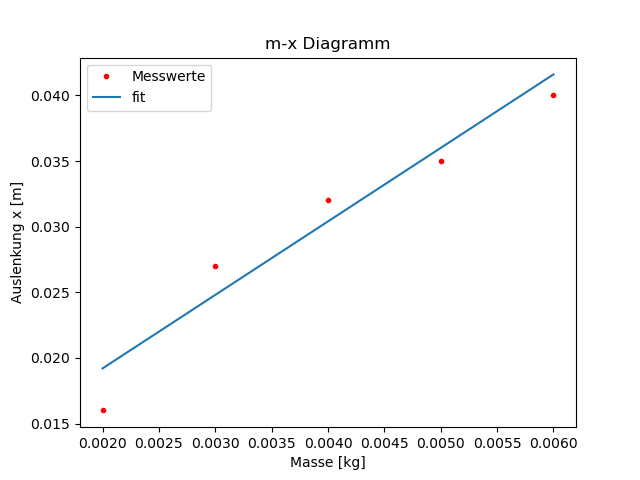
\includegraphics{1.png}

\noindent Die Ausgleichsgerade hat die Form $y=mx+n$.
Die Parameter wurden mit der Python erweiterung "curve fit" und die dazugehörigen Unsicherheiten,
mit der Erweiterung "uncertainties" berechnet.

\noindent Die Parameter haben folgende Werte:

\begin{center}
    \begin{tabular}{ll@{${}\pm{}$}l}
        \toprule
         & Wert & Unsicherheit \\
        \midrule
        a & 5.6 & 0.825 \\
        b & 0.008 & 0.003 \\
        \bottomrule 
    \end{tabular}
\end{center}


\noindent Die Federkonstante lässt sich mit Folgender Formel berechnen:

\begin{displaymath}
    k=\frac{g}{a}
\end{displaymath}

\noindent Für k ergibt sich $1.75 \pm 0.26$.

\section{Aufgabe 2}
\subsection{Aufgabe 2a}

Um die Brennweite f zu berechnen muss die Linsengleichung umgestellt werden.
Aus der Linsengleichung ergibt sich:

\begin{displaymath}
    f=\frac{g*b}{g+b}
\end{displaymath}

\noindent Diese Formel liefert folgende Brennweiten:
\begin{center}
    \begin{tabular}{lll}
        \toprule
        g & b & f \\
        \midrule
        60      & 285  & 49.565\\
        80      & 142  & 51.171\\
        100     & 117  & 53.917\\
        110     & 85   & 47.948\\
        120     & 86   & 50.097\\
        125     & 82   & 49.516\\
        \bottomrule 
    \end{tabular}
\end{center}

\noindent Der Mittelwert von f ist: 50.369

\noindent Die Standardabweichung wurde nach der Formel
\begin{displaymath}
    s = \sqrt{s^2} = \sqrt{\frac{1}{n-1} \sum_{i=1}^{n} (x_i - \bar{x})^2}
\end{displaymath}
berechnet.

\noindent Das Ergebnis ist: 1.8500

\noindent Der Fehler des Mittelwertes lässt sich berechnen durch:

\begin{displaymath}
    s_m=\frac{s}{\sqrt{n}}
\end{displaymath}

\noindent n ist in diesem Fall 6 und mit der ermittelten Standardabweichung ergibt sich $s_m=0.7552$

\noindent Der vollständige Mittelwert ist also 50.369$\pm$0.7552.

\subsection{Aufgabe 2b}

Das G-B Diagramm sieht folgendermaßen aus:

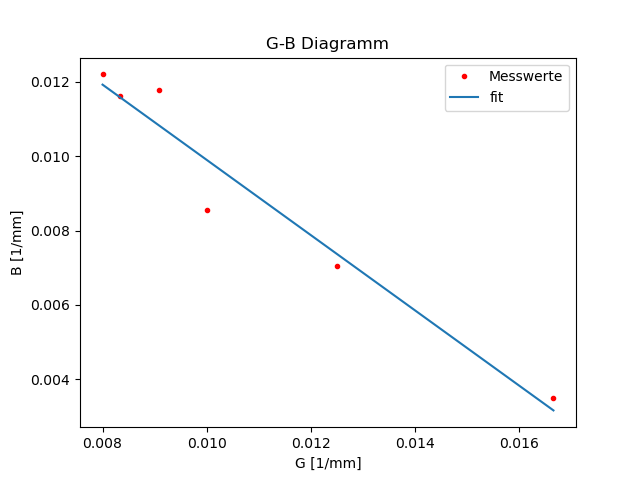
\includegraphics{2.png}

Die lineare Regression mit Python liefert eine Funktion der Form: 
\begin{displaymath}
    \frac{1}{b}=\frac{1}{g}a + b
\end{displaymath}

Mit den Parametern a=-1$\pm$0.118 und b=0.02$\pm$0.001

Diese Gleichung lässt sich umstellen zu:
\begin{displaymath}
    -\frac{b}{a} = \frac{1}{g} - \frac{1}{b*a}
\end{displaymath}

Mit a=-1 ergibt sich:
\begin{displaymath}
    f = \frac{1}{b}
\end{displaymath}

Daraus folgt: $f=50\pm2.5$.

\subsection{Aufgabe 2c}

Die relative Abweichung der beiden Werte für die Brennweite lässt sich berechnen durch:

\begin{displaymath}
    \Delta r = \frac{f_{formel}-f_{graphisch}}{f_{formel}}*100
\end{displaymath}

\noindent Es ergibt sich eine relative Abweichung der beiden Werte von 1\%.
Zwei verschiedene Ansätze der Bestimmung der Brennweite liefern also nahezu den gleichen Wert.
Der graphische Ansatz liefert eine Brennweite mit einem höheren Fehler.
Dieser entsteht dadurch, dass die Abweichung bei einer linearen Regression größer ist als bei den Rechnungen mit der Linsengleichung.
Nun wird dieser Unterschied allerdings nur relevant, wenn mit der Brennweite weitergerechnet werden soll.
Wenn das Ziel lediglich ist die Brennweite zu bestimmen sind beide Wege gleichwertig, da die Abweichung bei nur 1\% liegt.
Wenn mit der Brennweite allerdings weitergerechnet werden soll, sollte darauf geachtet werden, dass der größere Fehler, durch die Fehlerfortpflanzung,
noch größer wir. 
In diesem Fall sollte also der Ansatz über die Linsengleichung gewählt werden.

\section{Aufgabe 3}

Zuerst sollen bei dieser Aufgabe die Messunsicherheiten für N bestimmt werden.
Dies lässt sich umsetzen, indem lediglich die Quadratwurzel aus N gezogen wird ($\Delta N = \sqrt{N}$).

\noindent Diese Messunsicherheiten sind nocheinmal in folgender Tabelle zu sehen:
\begin{center}
    \begin{tabular}{lll}
        \toprule
        d [cm] & N [1/60s] & $\Delta N$ \\
        \midrule
        0.1  &   7565 & 86.97700846 \\
        0.2  &   6907 & 83.108363   \\
        0.3  &   6214 & 78.8289287  \\
        0.4  &   5531 & 74.37069315 \\
        0.5  &   4942 & 70.29935988 \\
        1.0  &   2652 & 51.49757276\\
        1.2  &   2166 & 46.54030511 \\
        1.5  &   1466 & 38.28837944 \\
        2.0  &    970 & 31.144823   \\
        3.0  &    333 & 18.24828759 \\
        4.0  &    127 & 11.26942767  \\
        5.0  &     48 & 6.92820323\\ 
        \bottomrule
    \end{tabular}  
\end{center}

\noindent Diese Werte können nun in einem Diagramm veranschaulicht werden.

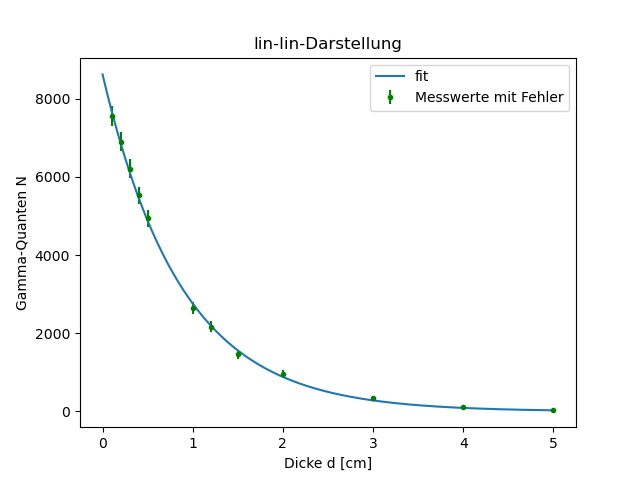
\includegraphics{3.png}

\noindent In diesem Fall ist ein Diagramm mit linearer Darstellung zu sehen. 
Mit zunehmender Dicke nimmt die Anzahl der Gamma-Quanten exponentiell ab.

\noindent Mit einer halblogarithmischen Darstellung ergibt sich folgendes Bild:

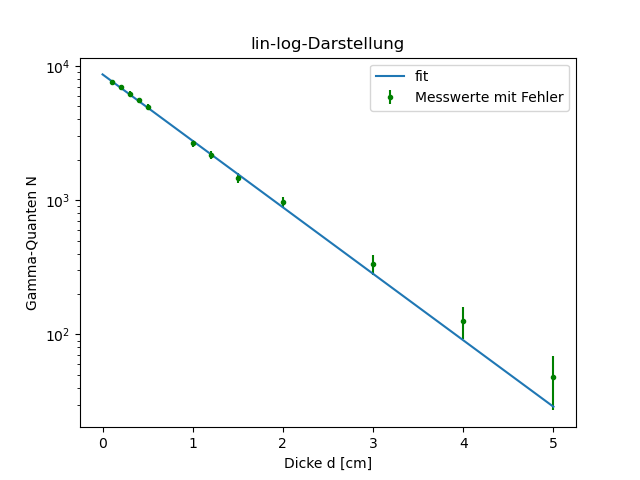
\includegraphics{4.png}

\noindent Durch die logarithmische Skala der y-Achse erscheint das Bild linear.

\noindent Die Ausgleichsrechnung mit einer Funktion der Form:
\begin{displaymath}
    N= N_0*e^{-µd}
\end{displaymath}
liefert einen Wert für alle Parameter.
Für den Parameter µ, den Absorptionskoeffizienten, ergibt sich:
\begin{displaymath}
    µ=1.139\pm0.019
\end{displaymath}

\end{document}